\documentclass[a4paper]{article}
\usepackage{minted}

\usepackage{polski}
\usepackage[utf8]{inputenc}

\usepackage[export]{adjustbox}
\usepackage{scrextend}
\usepackage{amsfonts}
\usepackage{amsmath}


\usepackage{geometry}
\geometry{a4paper, left=15mm, top=30mm, right=15mm, bottom=20mm}

\usepackage{gensymb}
\usepackage{graphicx} 
\usepackage{isotope}
\usepackage{array}
\usepackage{float}
\usepackage{titlesec}
\usepackage{fancyhdr}
\usepackage{multirow}

\usepackage{hyperref}
\usepackage{sectsty}
\usepackage{enumitem}
\usepackage{listings}
\usepackage[labelformat=simple]{subcaption}
\usepackage{xcolor,colortbl}


\usepackage{tikz}
\usetikzlibrary{shapes.geometric, arrows}
\tikzstyle{startstop} = [
    rectangle, 
    rounded corners, 
    minimum width=3cm, minimum height=1cm,
    text centered,
    draw=black, fill=red!30]
\tikzstyle{io} = [
    trapezium, trapezium left angle=70, trapezium right angle=110, 
    minimum width=3cm, minimum height=1cm, 
    text centered, 
    draw=black, fill=blue!30]
\tikzstyle{process} = [
    rectangle, 
    minimum width=3cm, minimum height=1cm, 
    text centered, 
    draw=black, fill=orange!30]
\tikzstyle{decision} = [
    diamond, 
    minimum width=3cm, minimum height=1cm, 
    text centered, 
    draw=black, fill=green!30]
\tikzstyle{arrow} = [thick,->,>=stealth]

\usepackage{karnaugh-map}

\sectionfont{\normalfont\huge\sectionrule{0pt}{0pt}{-6pt}{1pt}}
\subsectionfont{\normalfont\LARGE}
\subsubsectionfont{\normalfont\Large}

\pagestyle{fancy}
\fancyhf{}
\fancyhead[LE,LO]{\Large Łukasz Kwinta, Kacper Kozubowski, Ida Ciepiela}
\fancyhead[LE,RO]{\Large Układ FPGA}
\fancyfoot[CE,CO]{\Large\thepage}

\renewcommand{\footrulewidth}{1pt}
\renewcommand{\headrulewidth}{1pt}

\definecolor{Gray}{gray}{0.85}
\definecolor{LightGray}{gray}{0.95}

\newcolumntype{a}{>{\columncolor{Gray}}c}
\newcolumntype{b}{>{\columncolor{white}}c}

\hypersetup{
    colorlinks,
    citecolor=black,
    filecolor=black,
    linkcolor=black,
    urlcolor=black
}

\counterwithin{table}{section}
\counterwithin{figure}{section}

\title{\fontsize{30pt}{30pt}\selectfont Laboratorium 4 \\ Układ FPGA}
\author{\fontsize{20pt}{20pt}\selectfont Łukasz Kwinta, Kacper Kozubowski, Ida Ciepiela}
\date{maj 2024}

\begin{document}
\maketitle
\pagebreak
\large
\tableofcontents

\pagebreak
\section{Cel zadania}
\Large
Celem laboratorium było zaprogramowanie układu FPGA tak aby wyświetlał animację poruszających się 
segmentów na obrzeżach wyświetlaczy 7 segmentowych. Należało również, zaimplementować prostą funkcjonalność 
obejmującą zmianę prędkości i kierunku ruchu, świetlnego odcinka, przy pomocy znajdujących się na płytce przycisków.  

\section{Czym są układy FPGA?}
FPGA (Field-Programmable Gate Array) to rodzaj układu logicznego,
który można programować po jego wyprodukowaniu. W przeciwieństwie do tradycyjnych układów ASIC (Application-Specific Integrated Circuit), 
które są zaprojektowane do wykonywania jednego konkretnego zadania i nie mogą być zmieniane po wyprodukowaniu, 
FPGA oferują elastyczność i możliwość wielokrotnego programowania. 
Kluczowym aspektem takiego układu jest matryca programowalnych bloków logicznych i konfigurowalnych połączeń.

Bloki logiczne to podstawowe jednostki wykonujące logikę i arytmetykę.
Każdy blok zawiera programowalne elementy, takie jak bramki logiczne,
multiplexery, oraz przerzutniki, które można konfigurować do wykonywania różnych funkcji.
Natomiast, sieć połączeń umożliwia łączenie tych bloków w dowolny sposób.

Dzięki takiej konstrukcji układy FPGA można dostosować do różnych zastosowań, 
co czyni je niezwykle wszechstronnymi w inżynierii cyfrowej.

\pagebreak
\section{Realizacja}
Do napisania programu na układ FPGA, spełniającego warunki zadania, wykorzystaliśmy język opisu sprzętu Verilog, a także
oprogramowanie Vivado ML Edition od firmy Xilin.
Dostarczone przez nas rozwiązanie zostało przygotowane na płytkę Nexys-A7 50T.

\begin{figure}[H]
    \centering
    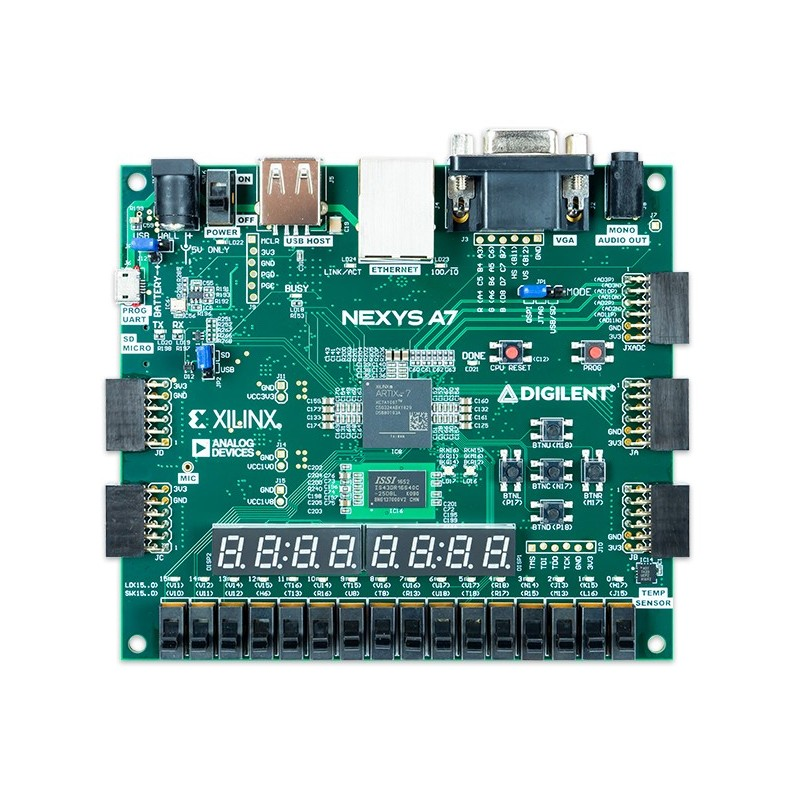
\includegraphics[width=\textwidth]{nexys-a7-artix-50t-fpga-xilinx-edu.jpg}
    \caption{Wykorzystana płytka z układem FPGA}
\end{figure}

\section{Rozwiązanie}
\begin{figure}[H]
    \centering
    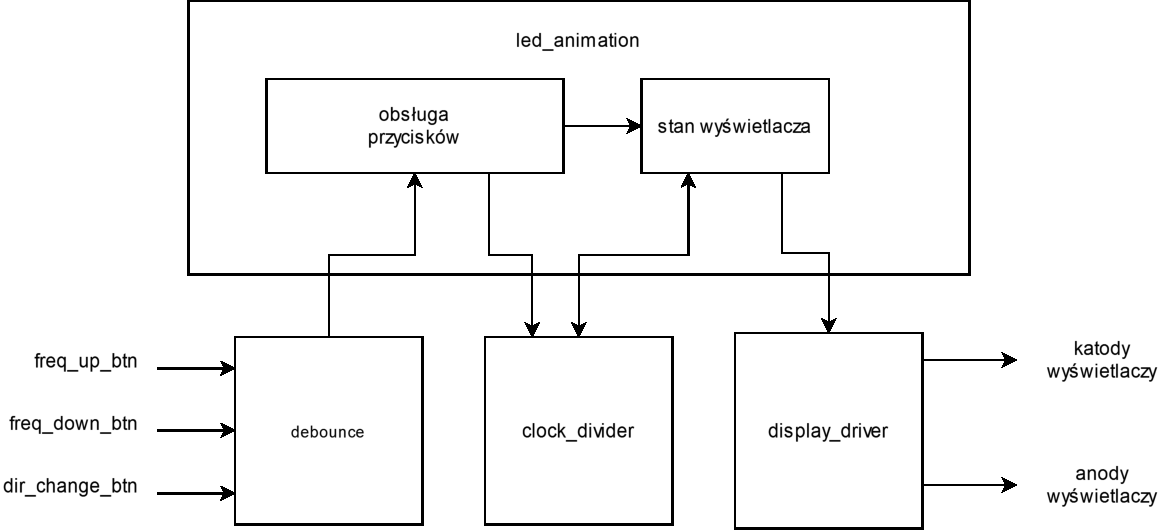
\includegraphics[width=\textwidth]{led_animation.drawio.pdf}
    \caption{Schemat blokowy rozwiązania}
\end{figure}
\subsection{Moduł dzielnika częstotliwości}
Aby w łatwy sposób zmieniać prędkość animacji, zdecydowaliśmy się na zastosowanie modułu dzielnika częstotliwości.
Moduł przyjmuje na wejściu zegar systemowy oraz rejestr oznaczający obecny okres
zegara wyjściowego. Następnie zlicza on takty zegara systemowego i gdy licznik dojdzie
do zadanej wartości, zmienia stan zegara wyjściowego na przeciwny.
\begin{minted}[
    frame=lines,
    framesep=2mm,
    baselinestretch=1.2,
    bgcolor=LightGray,
    fontsize=\footnotesize,
    linenos
]{verilog}
// moduł dzielący zegar
module clock_divider(
    input integer clock_period,
    input wire clk,
    
    output reg divided_clock
);


initial
    divided_clock <= 0;

longint counter_value = 0;

// zliczamy zadany okres zegara (ilość cykli zegara wejściowego), i gdy 
// doliczymy do konca zmieniamy stan spowolnionego zegara na przeciwny
always@ (posedge clk)
begin 
    if (counter_value >= clock_period) 
        begin
            divided_clock <= ~divided_clock;
            counter_value <= 0;
        end
    else 
        begin
            divided_clock <= divided_clock;
            counter_value <= counter_value + 1;
        end
end

endmodule
\end{minted}
\subsection{Moduł filtrujący przyciski}
Aby uniknąć efektu drgania styków przycisków, zdecydowaliśmy się na zastosowanie modułu
filtrującego wejście przycisków. Działa on na bardzo prostej zasadzie - zlicza on ilość 
cykli zegara systemowego w których przycisk jest w stanie wysokim - wciśnięty. Gdy ilość
cykli przekroczy zadaną wartość, przycisk uznawany jest za wciśnięty. Każdy stan niski 
pomiędzy kolejnymi resetuje licznik. Długość odliczania można ustawić poprzez
parametr DEBOUNCE\_TIME przy instancjonowaniu modułu.
\begin{minted}[
    frame=lines,
    framesep=2mm,
    baselinestretch=1.2,
    bgcolor=LightGray,
    fontsize=\footnotesize,
    linenos
]{verilog}
// moduł filtrujący przyciski
module debounce #(parameter DEBOUNCE_TIME = 1000 * 100) (
    input wire clk,
    input wire button_physical,
    
    output reg button_active
);

// ustawiamy początkowy stan przycisku na 0
initial
    button_active = 0;

integer btn_clock_cycles_counter = 0;

// zliczamy zadaną ilość cykli zegara 
// jeśli w którymś cyklu przycisk będzie w stanie niskimi,
// resetujemy licznik wartości
always@ (posedge clk)
begin
   if (button_physical == 1)
       begin
            btn_clock_cycles_counter <= btn_clock_cycles_counter + 1;
            if (btn_clock_cycles_counter >= DEBOUNCE_TIME) 
                button_active <= 1;
       end
    else 
        begin
            btn_clock_cycles_counter <= 0;
            button_active <= 0;
        end
        
end

endmodule
\end{minted}
\subsection{Moduł sterujący wyświetlaczami}
Aby wyświetlać wiele segmentów wielu wyświetlaczach 7 segmentowych na raz,
musieliśmy zaimplementować moduł sterujący wyświetlaczami. Moduł ten 
odświeża wyświetlacze z zadaną częstotliwością po kolei, tak aby 
stworzyć wrażenie, że wiele wyświetlaczy aktywnych jest w jednym czasie.

\begin{figure}[H]
    \centering
    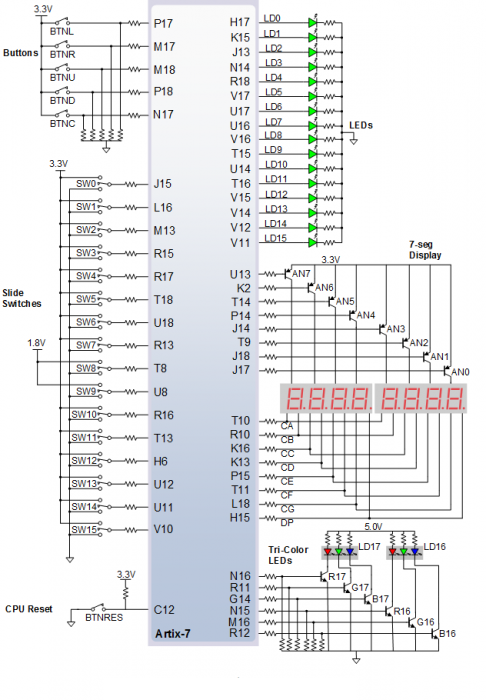
\includegraphics[width=0.6\textwidth]{fpga_led_diagram.png}
    \caption{Schemat podpięcia wyświetlaczy do układu FPGA}
\end{figure}

Zabieg ten musieliśmy zastosować gdyż wszystkie wyświetlacze 
mają wspólne katody segmentów co oznacza, że przy aktywacji 
anody wielu wyświetlaczy w jednym czasie, będą one wyświetlać te same 
segmenty.

\begin{minted}[
    frame=lines,
    framesep=2mm,
    baselinestretch=1.2,
    bgcolor=LightGray,
    fontsize=\footnotesize,
    linenos
]{verilog}
module displays_driver #(parameter REFERESH_PERIOD = 100 * 1000)(
    input wire clk,
    
    // rejestr wejściowy określający stan wszystkich wyświetlaczy
    input reg [7:0] display [7:0],
    
    // wyjscia steujace wyswietlaczami
    // stan niski na danym indeksie aktywuje dany wyswietlacz
    output reg [7:0] sseg_anodes,
    
    // |   7   |   6   |   5   |   4   |   3   |   2   |   1   |   0   |
    // |  DP   |   CG  |  CF   |  CE   |  CD   |  CC   |  CB   |  CA   |
    // stan niski na danym indeksie aktywuje dany segment na wszystkich aktywnych wyswietlaczach
    output reg [7:0] sseg_cathodes
);

initial 
begin
    sseg_anodes <= '1;
    sseg_cathodes <= '1;
end

reg refresh_clk; //1 khz refresh clock
clock_divider clk_div (
    .clock_period(REFERESH_PERIOD),
    .clk(clk),
    .divided_clock(refresh_clk)
);

reg [3:0] display_number = 0;

always@ (posedge refresh_clk)
begin 
    sseg_anodes = '1;
    sseg_anodes[display_number] <= 0;
    sseg_cathodes <= 8'(~display[display_number]);
    
    display_number = display_number + 1;
    if (display_number >= `DISPLAY_COUNT)
        display_number <= 0;
end

endmodule
\end{minted}
\subsection{Właściwy moduł generujący animację}
\begin{minted}[
    frame=lines,
    framesep=2mm,
    baselinestretch=1.2,
    bgcolor=LightGray,
    fontsize=\footnotesize,
    linenos
]{verilog}

\end{minted}

\section{Zastosowania układów FPGA}
\section{Wnioski}

\end{document}